
%!TEX TS-program = xelatex
%!TEX encoding = UTF-8 UnicodeWhat is at-issueness? An experimental comparison of diagnostics

\documentclass[compress, xcolor = dvipsnames, aspectratio=169]{beamer}

%fonts
	\usepackage{fontspec}
	\setmainfont[Scale=MatchLowercase,Mapping=tex-text]{Linux Biolinum}
	\setsansfont[Scale=MatchLowercase,Mapping=tex-text, BoldItalicFeatures={FakeBold=3}]{Linux Biolinum}
	\newfontfamily\opt{Optima}
	\usepackage{pifont}% http://ctan.org/pkg/pifont
	\newcommand{\cmark}{\ding{51}}%
	\newcommand{\xmark}{\ding{55}}%

%metadata
	\title{What is at-issueness?}
	\subtitle{An experimental comparison of diagnostics}
	\author{Conglei Xu, Lisa Hofmann, Judith Tonhauser}
	\institute{
\includegraphics[width=.3\textwidth]{../uni-logo-b.png}}
	\date{\small Experiments on the semantics/pragmatics interface (XPrag fest 2025)\\
	    	July 18st, 2025}

%theme
	\usetheme{default}
	\setbeamertemplate{navigation symbols}{}
	\setbeamertemplate{headline}{
		\begin{beamercolorbox}{section in head/foot}
			\vskip2pt\insertnavigation{\paperwidth}\vskip2pt
		\end{beamercolorbox}
	}
	\setbeamertemplate{footline}[frame number]

	\setbeamerfont{title}{family = \opt, series = \bfseries}
	\setbeamerfont{frametitle}{family = \opt, series = \bfseries}
	\setbeamerfont{headline}{family = \opt}

%color scheme
	% screen template
	\definecolor{bgyellow}{HTML}{FFFCF7}
	\definecolor{normaltext}{HTML}{505050}
	\definecolor{highlights}{HTML}{2a6d8c}

	\setbeamercolor{background canvas}{bg=bgyellow}
	\setbeamercolor{normal text}{fg=normaltext}
	\setbeamercolor{palette primary}{fg=highlights}
    \setbeamercolor{palette secondary}{fg=highlights}
    \setbeamercolor{palette tertiary}{fg=highlights}
    \setbeamercolor{palette quaternary}{fg=highlights}
    \setbeamercolor{structure}{fg=highlights}

    \setbeamertemplate{enumerate items}[circle]

% !TeX root = asymmetries-local-contexts.tex
%layout, formatting
	\usepackage[round]{natbib}
	\usepackage{multicol}
	\usepackage{linguex}
	\usepackage{multirow}
	\usepackage{colortbl}
	\usepackage{booktabs}
	\usepackage{array}
	\usepackage{hyperref}

%text features
	\usepackage{csquotes}
	\usepackage{stmaryrd}
	\usepackage[normalem]{ulem} % sout

%macros
	\newcommand{\listref}[1]{\phantom{.}\hfill {\scriptsize [#1]}}
	\newcommand{\transl}{\ensuremath\rightsquigarrow}

% drawing 
	\usepackage{tikz}
	\usepackage{venndiagram}
	\usepackage{easybmat}

% diagram shortcuts
	\usetikzlibrary{calc}
	\tikzstyle{index gray}=[inner sep=2pt, black, circle, fill=lightgray]
	\tikzstyle{opaque}=[fill=gray,fill opacity=.1]
	\newcommand{\indices}{% Indices
	    \draw (-1,1) node[index gray] (yy) {$w_{us}$};
	    \draw (1,1) node[index gray] (yn) {$w_u\phantom s$};
	    \draw (-1,-1) node[index gray] (ny) {$w_s\phantom u$};
	    \draw (1,-1) node[index gray] (nn) {$w_0\phantom i$};
		}


% propositions
	\newcommand{\sprop}{% s proposition
		\draw[rounded corners] (-1.9,1.9) rectangle (-.1, -1.9);}
	\newcommand{\uprop}{% u proposition
		\draw[rounded corners] (-1.9,1.9) rectangle (1.9,.1);}
	\newcommand{\nsprop}{% ~s proposition
		\draw[rounded corners] (1.9,-1.9) rectangle (.1, 1.9);}

% contexts
	\newcommand{\ccontext}{% c context
		\draw[opaque, rounded corners] (-1.8,1.8) rectangle (1.8, -1.8);}

	\newcommand{\ucontext}{% u context
		\draw[opaque, rounded corners] (-1.8,1.8) rectangle (1.8,.2);}
	\newcommand{\nucontext}{% ~u context
		\draw[opaque, rounded corners] (-1.8,-1.8) rectangle (1.8,-.2);}
	\newcommand{\scontext}{% s context
		\draw[opaque, rounded corners] (-1.8,1.8) rectangle (-.2, -1.8);}
	\newcommand{\nscontext}{% ~s context
		\draw[opaque, rounded corners] (1.8,1.8) rectangle (.2, -1.8);}
	
	\newcommand{\unscontext}{% u + ~s context
		\draw[opaque, rounded corners] (.2,1.8) rectangle (1.8,.2);}
	\newcommand{\uscontext}{% u + s context
		\draw[opaque, rounded corners] (-.2,1.8) rectangle (-1.8,.2);}
	\newcommand{\nuscontext}{% ~u + s context
		\draw[opaque, rounded corners] (-.2,-1.8) rectangle (-1.8,-.2);}
	\newcommand{\zerocontext}{% u + ~s context
		\draw[opaque, rounded corners] (.2,-1.8) rectangle (1.8,-.2);}

	\newcommand{\undefined}{% undefined context
		\draw[thick, Magenta] (-1.9,1.9) -- (1.9,-1.9);
		\draw[thick, Magenta] (-1.9,-1.9) -- (1.9,1.9);}
	
	\newcommand{\negquitwoqud}{% c context
		\draw[opaque, rounded corners] (-1.8,1) -- (-1.8,1.8) -- (.1,1.8) -- (.1,.1) -- (1.8,.1) -- (1.8, -1.8) -- (-.1, -1.8) -- (-.1, -.1) -- (-1.8, -.1) -- (-1.8,1);}
	\newcommand{\nquitcontext}{% not quit context
		\draw[opaque, rounded corners] (-1.8,0) -- (-1.8,1.8) -- (-.2,1.8) -- (-.2,-.2) -- (.2,-.2) -- (1.8,-.2) -- (1.8, -1.8) -- (-1.8, -1.8) -- 
		(-1.8,0);}

% local contexts
	\newcommand{\uslocal}{% u+s local context
		\draw[rounded corners] (-1.8,1.8) rectangle (-.2,.2);}
	\newcommand{\unslocal}{% u+~ns local context
		\draw[rounded corners] (1.8,1.8) rectangle (.2,.2);}
	\newcommand{\unslocalnudge}{% u+~ns local context
		\draw[rounded corners, xshift=-.1cm,yshift=-.1cm ] (1.8,1.8) rectangle (.2,.2);}
	

% input contexts
	\newcommand{\cinput}{% c input context
		\draw[dashed, rounded corners] (-1.9,1.9) rectangle (1.9, -1.9);}
	\newcommand{\uinput}{% u input context
		\draw[dashed, rounded corners] (-1.9,1.9) rectangle (1.9,.1);}
	\newcommand{\nuinput}{% u input context
		\draw[dashed, rounded corners] (-1.9,-1.9) rectangle (1.9,-.1);}
	\newcommand{\sinput}{% s input context
		\draw[dashed, rounded corners] (-1.9,1.9) rectangle (-.1, -1.9);}
	\newcommand{\nsinput}{% ~s input context
		\draw[dashed, rounded corners] (1.9,-1.9) rectangle (.1, 1.9);}


	% distance graph
	\newcommand{\distancegraph}{
    	\draw[->] (yn) -- (yy);   % yy → yn
    	\draw[->] (yn) -- (nn);   % yn → nn
	    \draw[->] (yy) -- (ny);   % yy → ny
	    \draw[->] (nn) -- (ny);   % ny → nn
        \draw (yn) circle (0.33);         % inner circle (node border is ~0.25 cm)
	    \draw (yn) circle (0.39);
		}
	\newcommand{\classes}{	
		\draw[shorten <= -1cm, shorten >= -1cm] ($(yy)!0.5!(yn)$) -- ($(yn)!0.5!(nn)$);
		\draw[shorten <= -1cm, shorten >= -1cm] ($(yy)!0.5!(ny)$) -- ($(ny)!0.5!(nn)$);}
	\newcommand{\classlabels}{
		\node at ($(yn)+(0.8,0.5)$) {$d=0$};                 % region containing w_u
		\node at ($(yy)!0.5!(nn)$)   {$d=1$};                 % region containing w_{us}, w_0
		\node at ($(ny)+(-0.8,-0.5)$){$d=2$}; 
	}




\begin{document}

\begin{frame}
\titlepage

\end{frame}

\section{Introduction}
	\begin{frame}\frametitle{At-issueness}\small
		Distinguish propositional content expressing the main point of an utterance (at-issue content) from those conveying background information (not-at-issue content) \pause

		\ex. \emph{Greg, who bought a new car, is envied by his neighbor.}
			\a. At-issue content: \emph{Greg is envied by his neighbor}
			\b. Not-at-issue content: \emph{Greg bought a new car}\pause
			\z.\z.
		
		\begin{itemize}
			\item Several definitions and diagnostics have been proposed in the literature\pause

			\item Very little discussion of whether definitions and diagnostics target the same underlying phenomenon (\citealt{snider_anaphoric_2017,snider_at-issuenessne_2017,snider_distinguishing_2018,koev_notions_2018,faller_discourse_2019,korotkova_evidential_2020})\pause

			\item This work: take a step in adressing this question, compare whether four commonly used diagnostics yield the same results for propositional contents introduced by the same kinds of expressions

			% \item exp 1--4 overview

		\end{itemize}
	
	\end{frame}

	\begin{frame}\frametitle{Experiments 1–4}
		\begin{itemize}
			\item Across four experiments, we manipulated the diagnostic used to assess the at-issueness status of the same contents\pause

			\item We chose four diagnostics that have been suggested to target different notions of at-issueness and show different empirical patterns (\citealt{snider_anaphoric_2017,snider_at-issuenessne_2017,snider_distinguishing_2018,koev_notions_2018,faller_discourse_2019,korotkova_evidential_2020})\pause

			\item We offer a systematic experimental comparison

		\end{itemize}
			
	\end{frame}

	\begin{frame}[t]\frametitle{Question-based at-issueness diagnostics}\small

		Question-based diagnostics assume a conception of at-issueness relative to the QUD: At-issue content is the part of an utterance that interacts with the current QUD (\citealt{amaral_review_2007,simons_what_2010})\pause

		\ex. \label{qud}%
		    QUD diagnostic (e.g., \citealt{tonhauser_diagnosing_2012,chen_presuppositions_2024})
		    \a.[A:] \emph{What did Greg buy?}
		    \b.[B:] \emph{Greg, who bought a new car, is envied by his neighbor.}
		    \z.
		    Question to participants: How well does B's response fit A's question?\pause
		\z.	

		\ex. \label{aw}%
		    `asking whether' diagnostic (e.g., \citealt{tonhauser_how_2018,solstad_cataphoric_2024})\smallskip\\
		      \emph{Is Greg, who bought a new car, envied by his neighbor?}\smallskip
		  \\ Question to participants: Is the speaker asking whether Greg bought a new car?\pause
		  \z.

		\begin{itemize}
			\item Other diagnostics make other assumptions
			(\citealt{snider_anaphoric_2017,snider_at-issuenessne_2017,snider_distinguishing_2018,koev_notions_2018,faller_discourse_2019,korotkova_evidential_2020})
		\end{itemize}
	
	\end{frame}

	\begin{frame}[t]\frametitle{Assertion-based at-issueness diagnostics}\small
		Assertion-based diagnostics assume that the at-issue content of an assertion constitues a proposal to update the common ground that can be affirmed or denied (\citealt{farkas_reacting_2010,murray_varieties_2014,anderbois_at-issue_2015})\pause

		  \ex. \label{dd} Direct dissent diagnostic (e.g., \citealt{tonhauser_diagnosing_2012,syrett_experimental_2015})
		    \a.[A:] \emph{Greg, who bought a new car, is envied by his neighbor.}
		    \b.[B:]\emph{No, that's not true, he didn't buy a new car.}
		    \z.
		  Question to participants: How natural is B's rejection of A's utterance?\pause
		  \z.

		  \ex. \label{yesbut}%
		    `yes, but' diagnostic (e.g., \citealt{xue_correlation_2011,destruel_cross-linguistic_2015})
		    \a.[A:] \emph{Greg, who bought a new car, is envied by his neighbor.}
		    \b.[B:] \emph{Yes, but he didn't buy a new car.} /
		    \b.[] \emph{Yes, and he didn't buy a new car.} /
		    \b.[] \emph{No, he didn't buy a new car.}
		    \z.
		    Task for participants: Choose the response that sounds best.
		  \z.
	
	\end{frame}

	\begin{frame}\frametitle{Experiments 1–4: contents}\small
		In seven conditions, each experiment tested propositional contents which previous literature leads us to expect show differences in at-issueness status\medskip\\ \pause

		Propositional contents associated with:
		\begin{itemize}
			\item Sentence-medial and sentence-final appositive NRRCs (non-restrictive relative clauses): \citealt{syrett_experimental_2015} found that final appositives are more at-issue than medial ones under a version of the direct-dissent diagnostic\pause

			\item Clauses embedded by \emph{be right, confirm, discover, confess,} and \emph{know}: \citealt{degen-tonhauser-glossa} found fine-grained differences in how at-issue these are under the `asking-whether' diagnostic\pause
		\end{itemize}

		In each experiment, 80 participants saw each of 7 conditions once, each randomly paired with a clause to instantiate it (item), e.g. \emph{Greg bought a new car}, + 2 controls (attention checks)
		
	\end{frame}

	\begin{frame}[t]\frametitle{Materials}\scriptsize
			
			\vspace{-2\baselineskip}
			\begin{center}
				\begin{tabular}{p{.3\linewidth} p{.3\linewidth}}	
					{\visible<1->{\centering Exp.~1 (QUD diagnostic)}} &
					{\visible<2->{\centering Exp.~2 (`asking whether' diagnostic)}} \\
					%
					\visible<1->{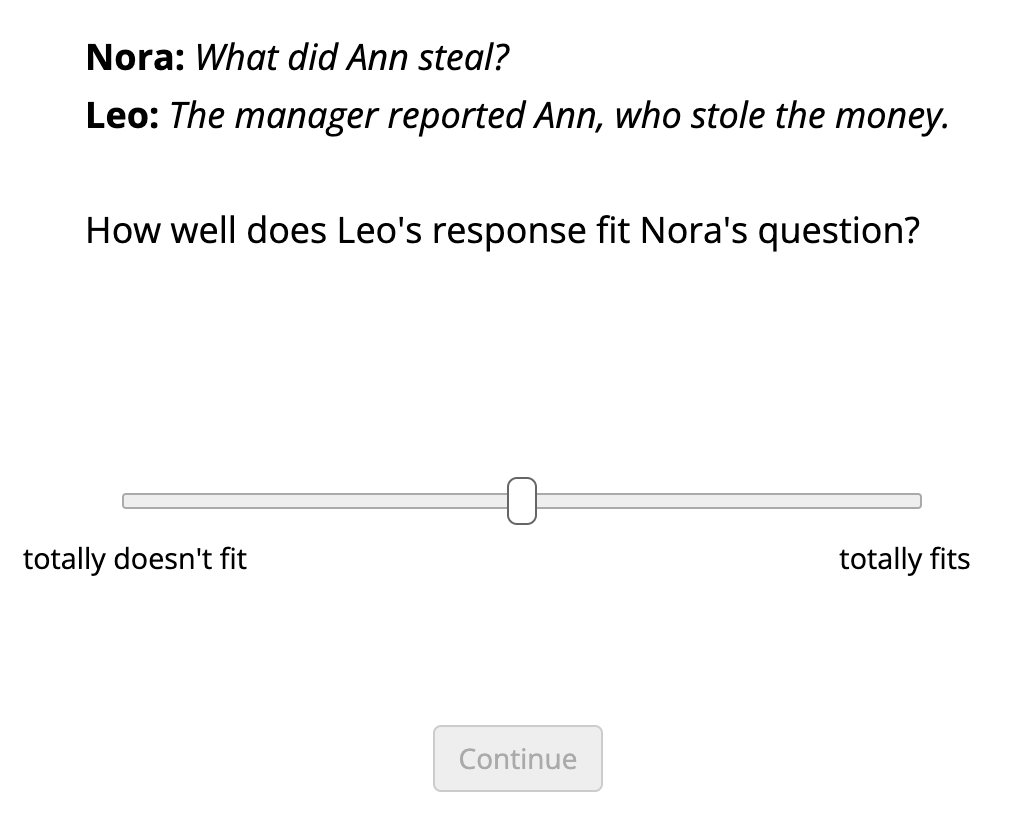
\includegraphics[width=\linewidth]{../../writing/paper/figures/trialExp1}}
					&
					\visible<2->{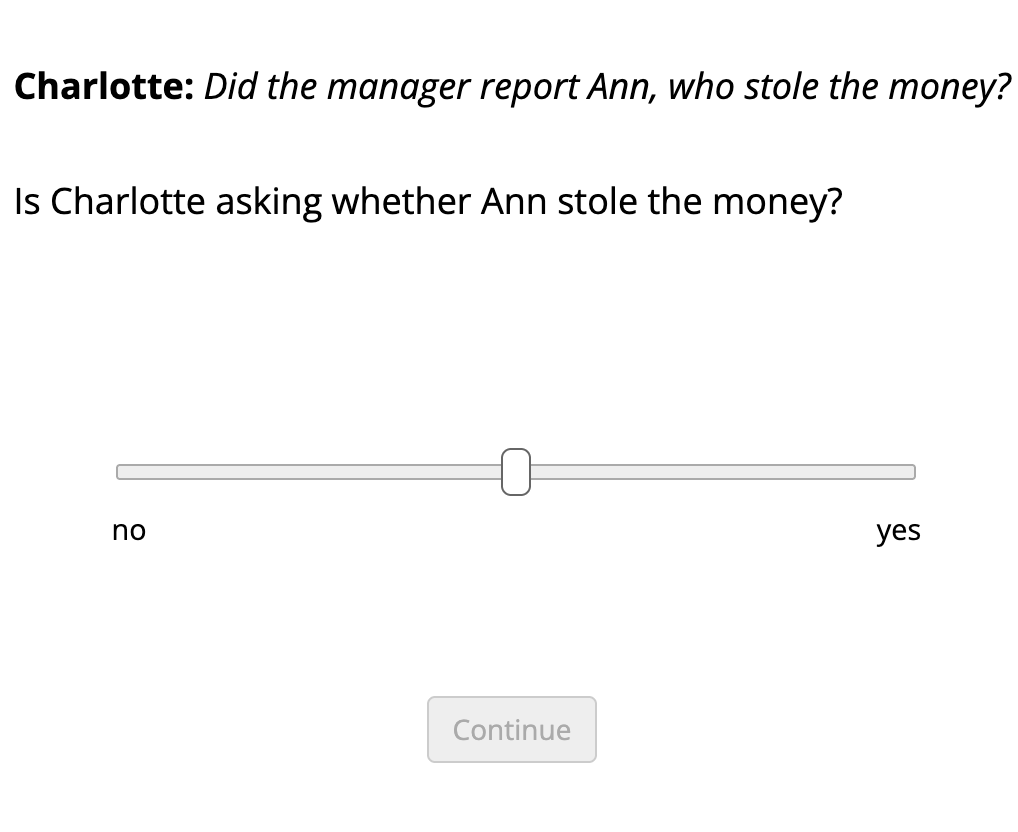
\includegraphics[width=\linewidth]{../../writing/paper/figures/trialExp2}}
					\\
					%
					{\visible<3->{\centering Exp.~3 (`direct dissent' diagnostic)}} &
					{\visible<4->{\centering Exp.~4 (`yes, but' diagnostic)}} \\
					%
					\visible<3->{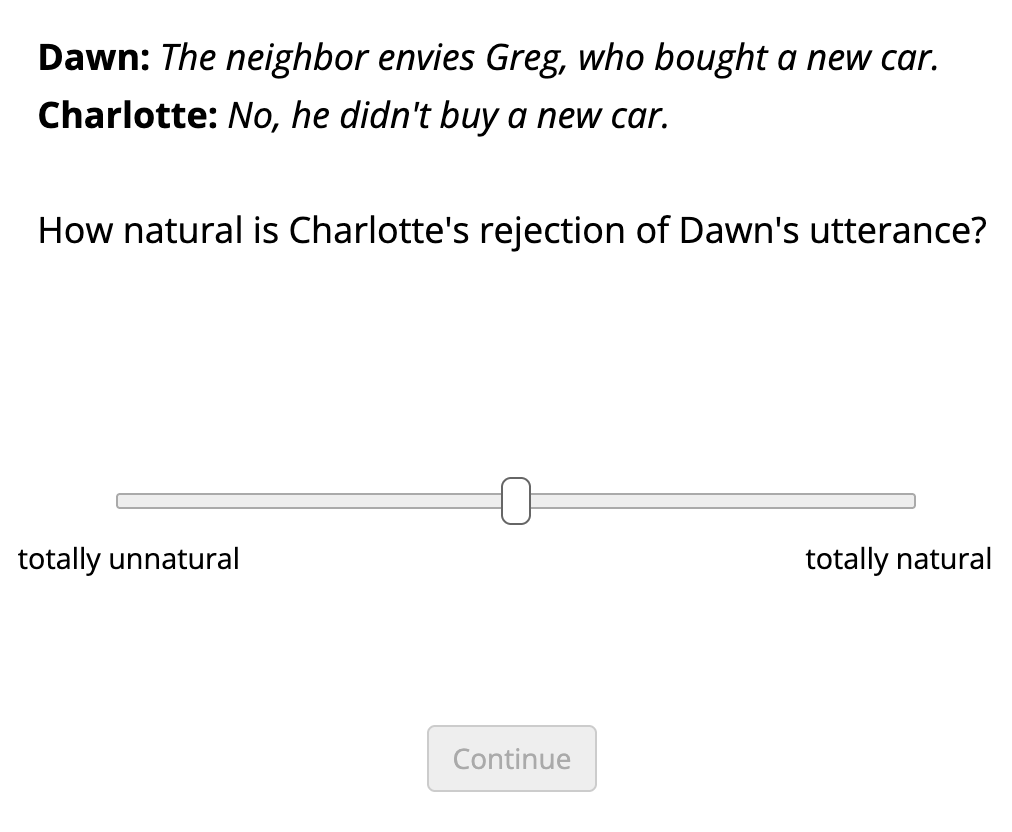
\includegraphics[width=\linewidth]{../../writing/paper/figures/trialExp3}}
					&
					\visible<4->{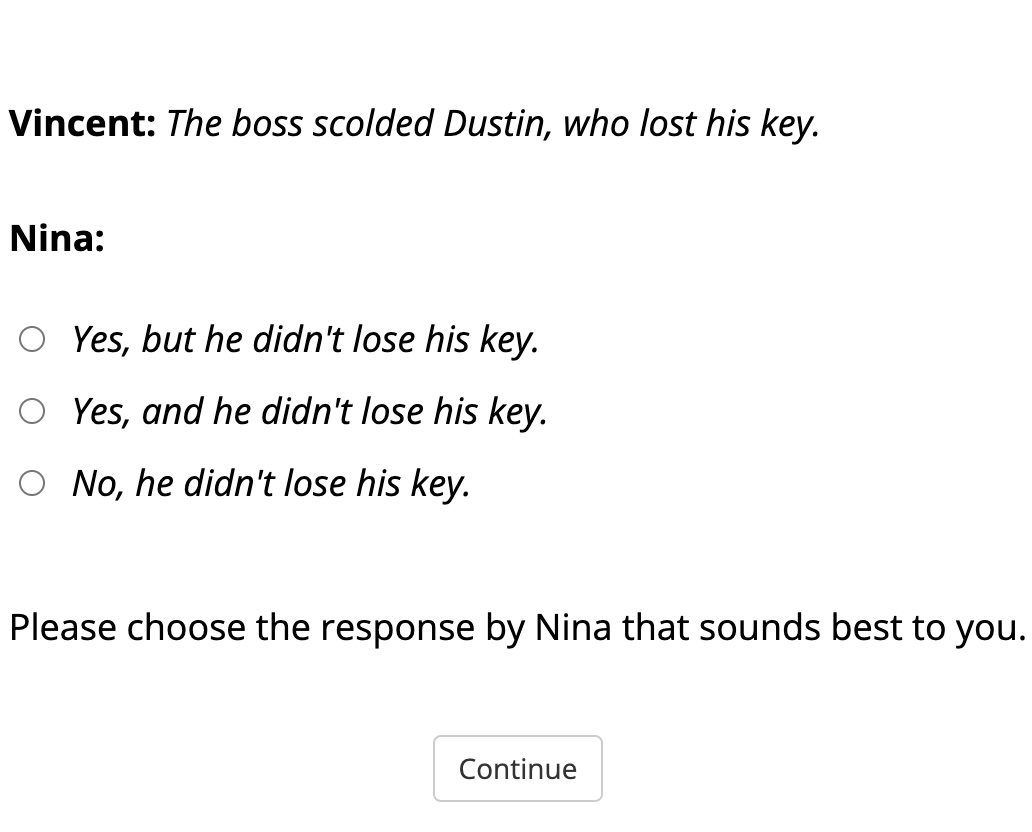
\includegraphics[width=\linewidth]{../../writing/paper/figures/trialExp4}}
					\\
				\end{tabular}
			\end{center}
			
	\end{frame}


\section{Experiments 1–4: Results}

	\begin{frame}[t]\frametitle{Results}\scriptsize
		\vspace{-.5\baselineskip}
		\begin{minipage}{\textwidth}
		\hspace{-1.18cm}
		\begin{minipage}{\textwidth}
			% \fbox{
			\begin{tabular}{p{.77\textwidth} p{.31\textwidth}}
				\begin{tabular}{p{.37\textwidth} p{.37\textwidth}}
					{\centering Exp.~1 (QUD diagnostic)} &
					{\centering Exp.~2 (`asking whether' diagnostic)} \\
		      		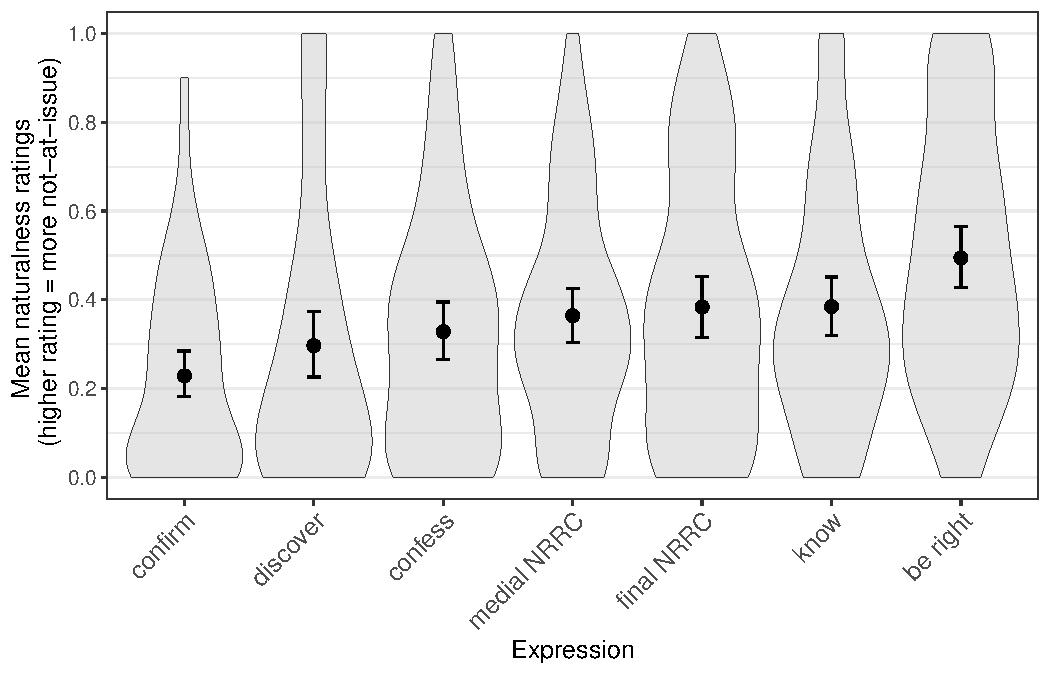
\includegraphics[width=\linewidth]{../../results/exp1/graphs/mean-ratings.pdf}
		      		&
		      		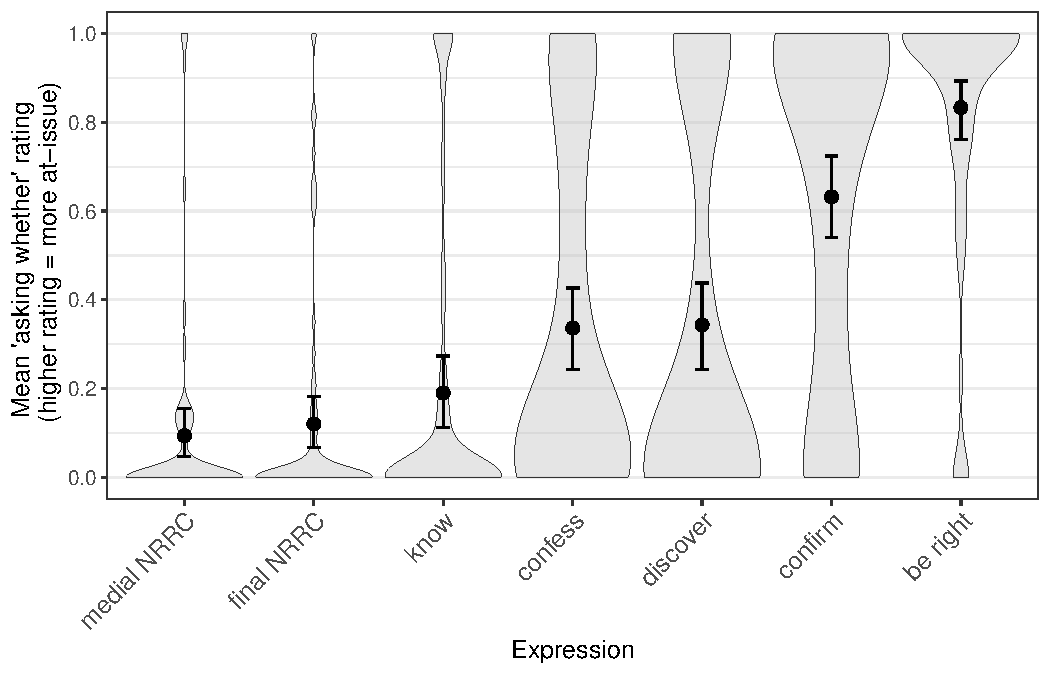
\includegraphics[width=\linewidth]{../../results/exp2/graphs/mean-ratings.pdf}
		      		\\
		      		{\centering Exp.~3 (`direct dissent' diagnostic)} &
					{\centering Exp.~4 (`yes, but' diagnostic)} \\
		      		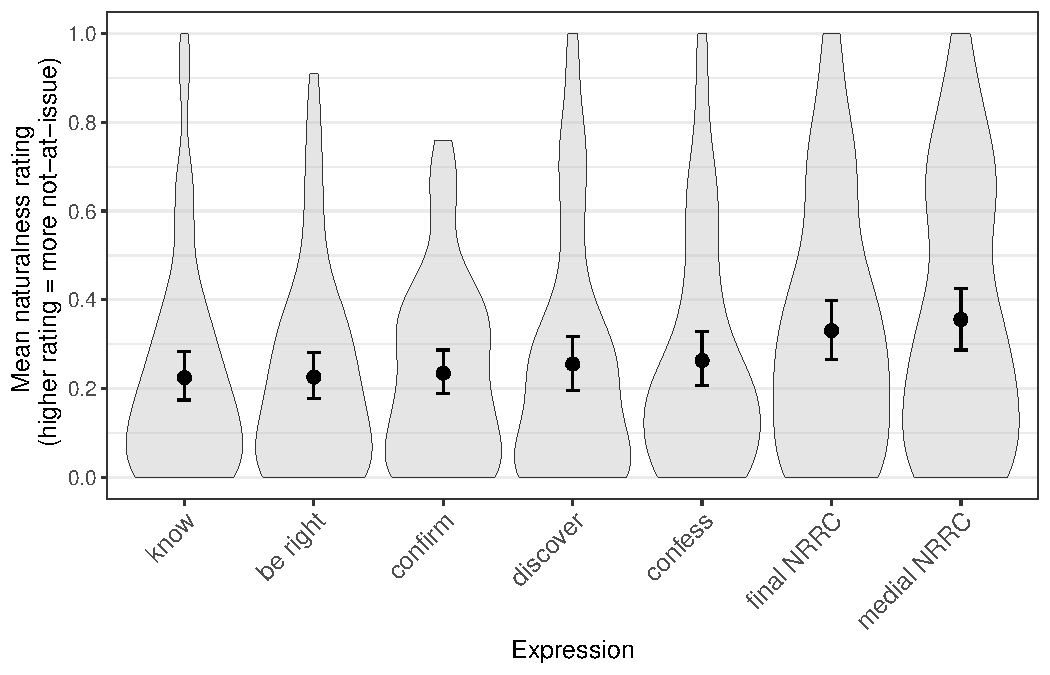
\includegraphics[width=\linewidth]{../../results/exp3/graphs/mean-ratings.pdf}
		      		&
		      		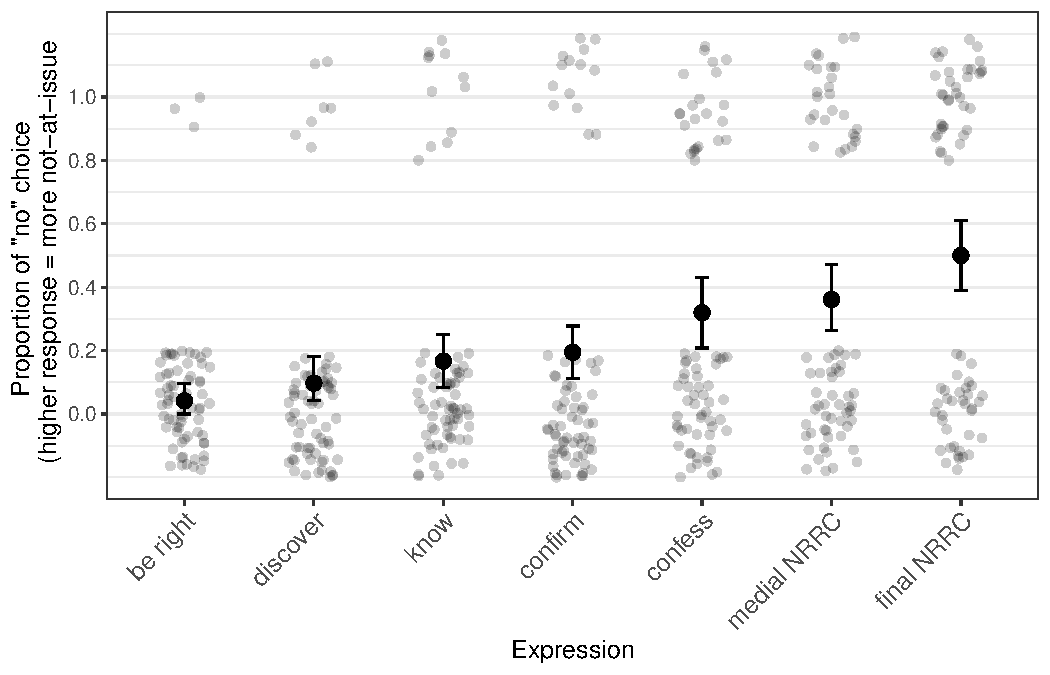
\includegraphics[width=\linewidth]{../../results/exp4/graphs/mean-ratings.pdf}
		      		\\
				\end{tabular}\pause

				&
				\parbox{\linewidth}{
				\parbox{\linewidth}{\scriptsize
				Exp.~2 (`asking whether'): greatest differentiation between contents
				\begin{itemize}
					\item Range of means
					\item More pairwise differences between contents\smallskip
				\end{itemize}

				\uncover<0>{Content rankings always different
				\begin{itemize}
					\item Embedded content of \emph{confirm} and \emph{discover} always more at-issue than NRRCs
					\item No other pairwise difference is found for all diagnostics\smallskip
				\end{itemize}

				Final NRRCs are not more at issue than medial NRRCs\medskip
				}
				\uncover<0>{\fbox{\parbox{\linewidth}{\tiny Posthoc pairwise comparisons of the estimated means/proportions for each content using the `emmeans' package (\citealt{emmeans}) in R (\citealt{r}). The input to the pairwise comparisons were bayesian mixed-effects beta regression models (Exps.~1-3) or a mixed-effects logistic regression model (Exp.~4)}}\\ \vfill \phantom. }}
				}
			\end{tabular}
			% }
		\end{minipage}
		\end{minipage}
	
	\end{frame}

	\begin{frame}[t]\frametitle{Results}\scriptsize
		\vspace{-.5\baselineskip}
		\begin{minipage}{\textwidth}
		\hspace{-1.18cm}
		\begin{minipage}{\textwidth}
			% \fbox{
			\begin{tabular}{p{.77\textwidth} p{.31\textwidth}}
				\begin{tabular}{p{.37\textwidth} p{.37\textwidth}}
					{\centering Exp.~1 (QUD diagnostic)} &
					{\centering Exp.~2 (`asking whether' diagnostic)} \\
		      		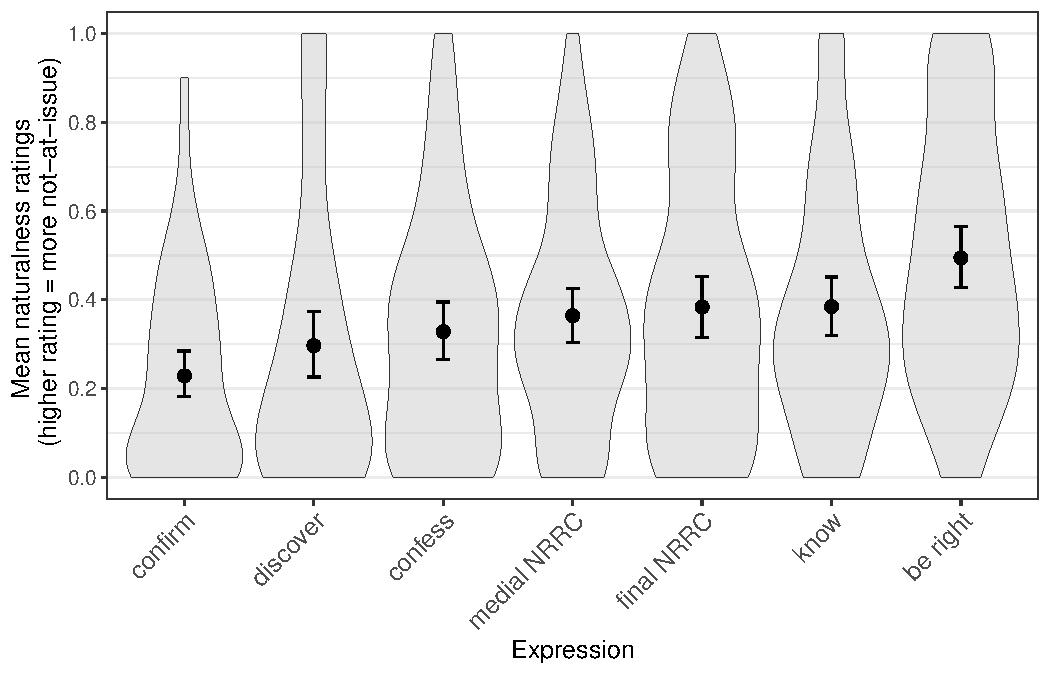
\includegraphics[width=\linewidth]{../../results/exp1/graphs/mean-ratings.pdf}
		      		&
		      		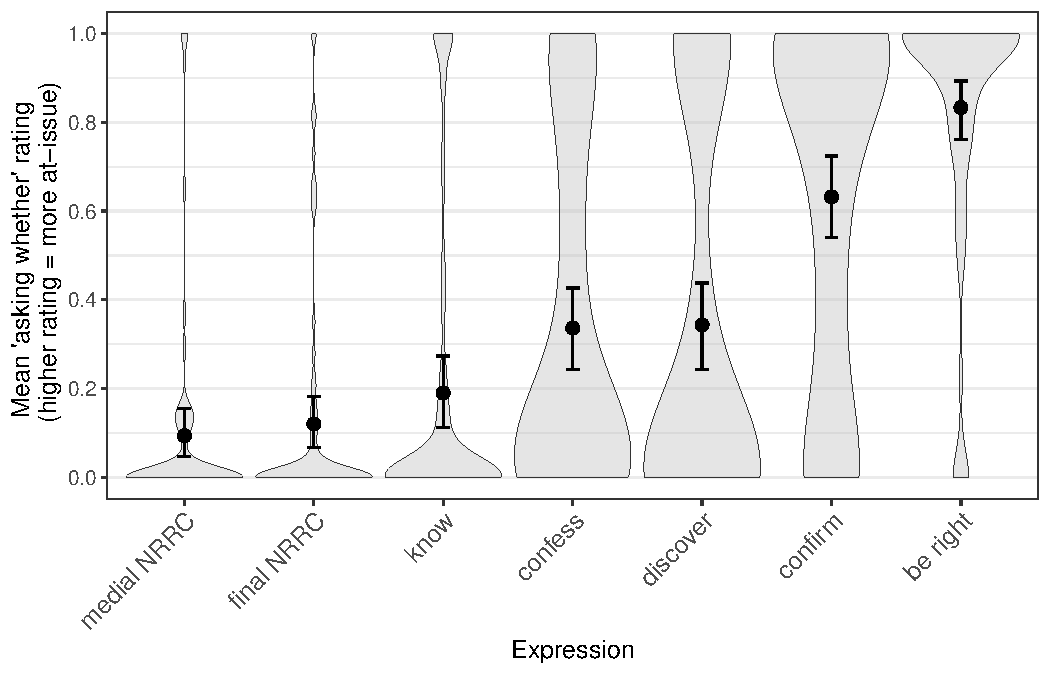
\includegraphics[width=\linewidth]{../../results/exp2/graphs/mean-ratings.pdf}
		      		\\
		      		{\centering Exp.~3 (`direct dissent' diagnostic)} &
					{\centering Exp.~4 (`yes, but' diagnostic)} \\
		      		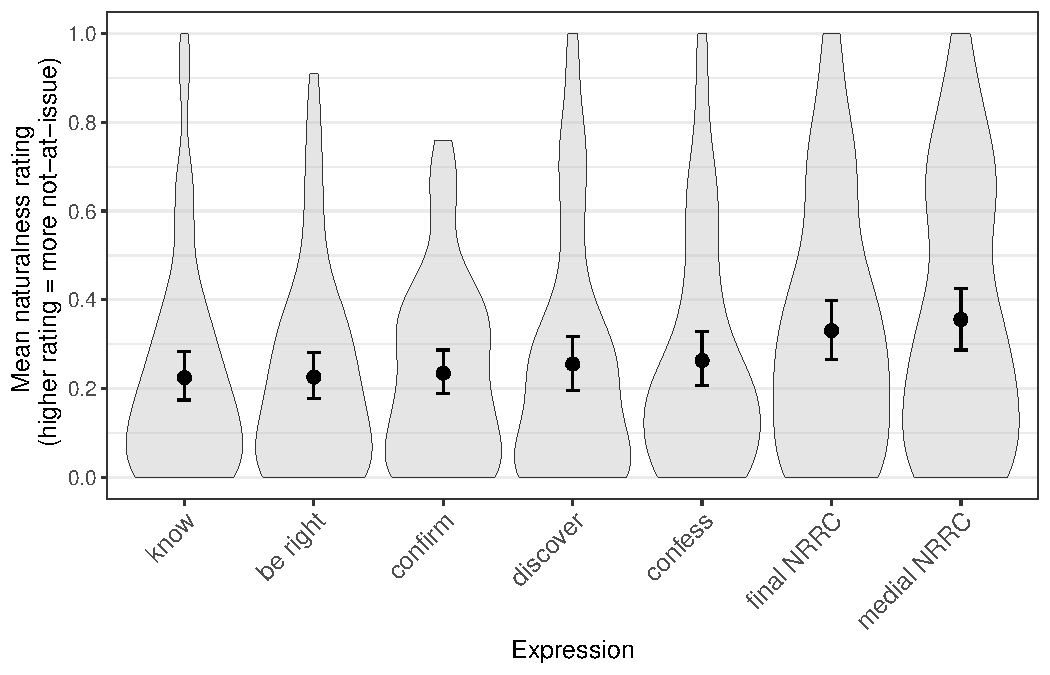
\includegraphics[width=\linewidth]{../../results/exp3/graphs/mean-ratings.pdf}
		      		&
		      		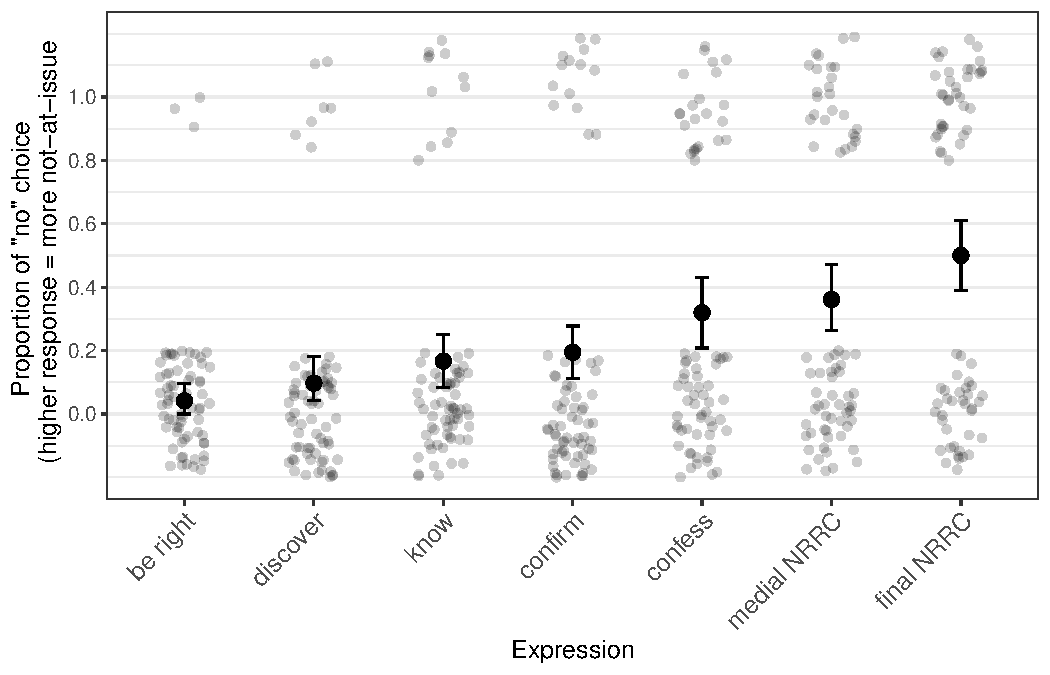
\includegraphics[width=\linewidth]{../../results/exp4/graphs/mean-ratings.pdf}
		      		\\
				\end{tabular}

				&
				\parbox{\linewidth}{
				\parbox{\linewidth}{\scriptsize
				Exp.~2 (`asking whether'): greatest differentiation between contents
				\begin{itemize}
					\item Range of means
					\item More pairwise differences between contents\smallskip
				\end{itemize}


				\uncover<2->{Content rankings always different
				\begin{itemize}
					\item Embedded content of \emph{confirm} and \emph{discover} always more at-issue than NRRCs
					\item No other pairwise difference is found for all diagnostics\smallskip
				\end{itemize}}

				\uncover<3->{Final NRRCs are not more at issue than medial NRRCs\medskip}
				}
				\fbox{\parbox{\linewidth}{\tiny Posthoc pairwise comparisons of the estimated means/proportions for each content using the `emmeans' package (\citealt{emmeans}) in R (\citealt{r}). The input to the pairwise comparisons were bayesian mixed-effects beta regression models (Exps.~1-3) or a mixed-effects logistic regression model (Exp.~4)}}\\ \vfill \phantom. 
				}
			\end{tabular}
			% }
		\end{minipage}

		\phantom.
		\hspace{-1.18cm}\begin{minipage}{\textwidth}
			\vspace{-8cm}
			% \fbox{
			\begin{tabular}{p{.77\textwidth} p{.31\textwidth}}
				\begin{tabular}{p{.37\textwidth} p{.35\textwidth}}
					\phantom{\centering Exp.~1 (QUD diagnostic)} &
					\phantom{\centering Exp.~2 (`asking whether' diagnostic)} \\
					%	
						\cellcolor{bgyellow}
						\parbox{\linewidth}{
						\vspace{.2cm}
						\scalebox{.75}{
			      		\begin{tabular}{r | ccccccc}
						    & \rots{be right} & \rots{confirm} & \rots{discover} & \rots{confess} & \rots{know} & \rots{final NRRC} & \rots{medial NRRC} \\
						    \hline
						     be right & \cellcolor{black} & \cellcolor{red} & \cellcolor{red} & \cellcolor{red} & \cellcolor{red} & \cellcolor{red} & \cellcolor{red} \\ 
  confirm & \cellcolor{black} & \cellcolor{black} & \cellcolor{white} & \cellcolor{blue} & \cellcolor{blue} & \cellcolor{blue} & \cellcolor{blue} \\ 
  discover & \cellcolor{black} & \cellcolor{black} & \cellcolor{black} & \cellcolor{white} & \cellcolor{white} & \cellcolor{blue} & \cellcolor{blue} \\ 
  confess & \cellcolor{black} & \cellcolor{black} & \cellcolor{black} & \cellcolor{black} & \cellcolor{white} & \cellcolor{white} & \cellcolor{white} \\ 
  know & \cellcolor{black} & \cellcolor{black} & \cellcolor{black} & \cellcolor{black} & \cellcolor{black} & \cellcolor{white} & \cellcolor{white} \\ 
  final NRRC & \cellcolor{black} & \cellcolor{black} & \cellcolor{black} & \cellcolor{black} & \cellcolor{black} & \cellcolor{black} & \cellcolor{white} \\ 
  medial NRRC & \cellcolor{black} & \cellcolor{black} & \cellcolor{black} & \cellcolor{black} & \cellcolor{black} & \cellcolor{black} & \cellcolor{black} \\ 
  

						    \hline
					    \end{tabular}}}
		      		&
		      			\cellcolor{bgyellow}
		      			\parbox{\linewidth}{
						\vspace{.2cm}
						\scalebox{.75}{
			      		\begin{tabular}{r | ccccccc}
						    & \rots{be right} & \rots{confirm} & \rots{discover} & \rots{confess} & \rots{know} & \rots{final NRRC} & \rots{medial NRRC} \\
						    \hline
						     be right & \cellcolor{black} & \cellcolor{blue} & \cellcolor{blue} & \cellcolor{blue} & \cellcolor{blue} & \cellcolor{blue} & \cellcolor{blue} \\ 
  confirm & \cellcolor{black} & \cellcolor{black} & \cellcolor{blue} & \cellcolor{blue} & \cellcolor{blue} & \cellcolor{blue} & \cellcolor{blue} \\ 
  discover & \cellcolor{black} & \cellcolor{black} & \cellcolor{black} & \cellcolor{white} & \cellcolor{blue} & \cellcolor{blue} & \cellcolor{blue} \\ 
  confess & \cellcolor{black} & \cellcolor{black} & \cellcolor{black} & \cellcolor{black} & \cellcolor{blue} & \cellcolor{blue} & \cellcolor{blue} \\ 
  know & \cellcolor{black} & \cellcolor{black} & \cellcolor{black} & \cellcolor{black} & \cellcolor{black} & \cellcolor{blue} & \cellcolor{blue} \\ 
  final NRRC & \cellcolor{black} & \cellcolor{black} & \cellcolor{black} & \cellcolor{black} & \cellcolor{black} & \cellcolor{black} & \cellcolor{white} \\ 
  medial NRRC & \cellcolor{black} & \cellcolor{black} & \cellcolor{black} & \cellcolor{black} & \cellcolor{black} & \cellcolor{black} & \cellcolor{black} \\ 
  

						    \hline
					    \end{tabular}}
					    \vspace{.1cm}
					    }
		      		\\
		      		\phantom{\centering Exp.~3 (`direct dissent' diagnostic)} &
					\phantom{\centering Exp.~4 (`yes, but' diagnostic)} \vspace{.05cm} \\
		      		%	
						\cellcolor{bgyellow}
						\parbox{\linewidth}{
						\vspace{.2cm}
						\scalebox{.75}{
			      		\begin{tabular}{r | ccccccc}
						    & \rots{be right} & \rots{confirm} & \rots{discover} & \rots{confess} & \rots{know} & \rots{final NRRC} & \rots{medial NRRC} \\
						    \hline
						     be right & \cellcolor{black} & \cellcolor{white} & \cellcolor{white} & \cellcolor{white} & \cellcolor{white} & \cellcolor{blue} & \cellcolor{blue} \\ 
  confirm & \cellcolor{black} & \cellcolor{black} & \cellcolor{white} & \cellcolor{white} & \cellcolor{white} & \cellcolor{blue} & \cellcolor{blue} \\ 
  discover & \cellcolor{black} & \cellcolor{black} & \cellcolor{black} & \cellcolor{white} & \cellcolor{white} & \cellcolor{blue} & \cellcolor{blue} \\ 
  confess & \cellcolor{black} & \cellcolor{black} & \cellcolor{black} & \cellcolor{black} & \cellcolor{white} & \cellcolor{white} & \cellcolor{blue} \\ 
  know & \cellcolor{black} & \cellcolor{black} & \cellcolor{black} & \cellcolor{black} & \cellcolor{black} & \cellcolor{blue} & \cellcolor{blue} \\ 
  final NRRC & \cellcolor{black} & \cellcolor{black} & \cellcolor{black} & \cellcolor{black} & \cellcolor{black} & \cellcolor{black} & \cellcolor{white} \\ 
  

						    \hline
					    \end{tabular}} \vspace{.1cm}}
		      		&
		      		%	
						\cellcolor{bgyellow}
						\parbox{\linewidth}{
						\vspace{.2cm}
						\scalebox{.75}{
			      		\begin{tabular}{r | ccccccc}
						    & \rots{be right} & \rots{confirm} & \rots{discover} & \rots{confess} & \rots{know} & \rots{final NRRC} & \rots{medial NRRC} \\
						    \hline
						     be right & \cellcolor{black} & \cellcolor{blue} & \cellcolor{white} & \cellcolor{blue} & \cellcolor{blue} & \cellcolor{blue} & \cellcolor{blue} \\ 
  confirm & \cellcolor{black} & \cellcolor{black} & \cellcolor{white} & \cellcolor{blue} & \cellcolor{white} & \cellcolor{blue} & \cellcolor{blue} \\ 
  discover & \cellcolor{black} & \cellcolor{black} & \cellcolor{black} & \cellcolor{blue} & \cellcolor{white} & \cellcolor{blue} & \cellcolor{blue} \\ 
  confess & \cellcolor{black} & \cellcolor{black} & \cellcolor{black} & \cellcolor{black} & \cellcolor{red} & \cellcolor{blue} & \cellcolor{white} \\ 
  know & \cellcolor{black} & \cellcolor{black} & \cellcolor{black} & \cellcolor{black} & \cellcolor{black} & \cellcolor{blue} & \cellcolor{blue} \\ 
  final NRRC & \cellcolor{black} & \cellcolor{black} & \cellcolor{black} & \cellcolor{black} & \cellcolor{black} & \cellcolor{black} & \cellcolor{red} \\ 
  medial NRRC & \cellcolor{black} & \cellcolor{black} & \cellcolor{black} & \cellcolor{black} & \cellcolor{black} & \cellcolor{black} & \cellcolor{black} \\ 
  

						    \hline
					    \end{tabular}}\vspace{.1cm}}
		      		\\
				\end{tabular}

				&
				\\ 
			\end{tabular}
			% }
		\end{minipage}
		\end{minipage}
	
	\end{frame}

	\begin{frame}\frametitle{Takeaways and quesions}
		\begin{itemize}
			\item We do see differences between diagnostics, importantly not all show the same differences between contents\pause

			\item None of our diagnostics replicate finding from \citet{syrett_experimental_2015} that final appositives are more at issue than medial ones\pause

			\item Only the `asking whether' diagnostic replicates finding from \citealt{degen-tonhauser-glossa} that clause-embedding predicates show fine-grained lexical differences in how at-issue the embedding clause is\pause

		\end{itemize}	\bigskip 

		We further explore this question:

		\begin{center}
			\emph{Why does Exp.~2 `asking whether' show a greater differentiation of contents than the other diagnostics?}
		\end{center}
		
	\end{frame}

	\begin{frame}[t]\frametitle{Why is `asking whether' so different?}\small 
		Previous literature:
		\begin{itemize}
			\item \textbf{Question-based vs. assertion-based at-issueness} diagnostics:\\
				The question-based diagnostics (QUD, `asking whether') are about whether a proposition is at issue relative to a QUD introduced in the previous discourse, wheras assertion-based diagnostics (direct dissent, `yes but') target a different underlying notion

		\end{itemize}\pause
		\vfill 

		Two other hypotheses: When testing a range of contents, the differentiation between contents (in terms of range of means, significant differences) is greater:
		\begin{enumerate}
			\item \textbf{Question embedding:} \\ 
				\dots when contents are embedded in a question vs. a declarative assertion.\pause
				
			\item \textbf{Response task:} \\ \dots when participants are more directly asked what the utterance was about vs. when giving acceptability judgment or forced-choice continuation responses.
			
		\end{enumerate}

	\end{frame}

\section{Experiments 5–6}

	\begin{frame}[t]\frametitle{Question-embedding or response task?}\scriptsize
	

		In experiments 5 and 6, we test whether the fine-grained differences among clause-embedding predicates observed with one diagnostic (asking-whether) are replicated with other diagnostics.

		\ex.
		    \a.\label{exp5} Exp.~5 (`asking whether' diagnostic )
		    \\ {\bf Nora:} \emph{Is Cole right that Lucy broke the plate?}
		    \\ Question to participants: Is Nora asking whether Lucy broke the plate?\smallskip
		    \b.\label{exp6} Exp.~6 (`direct response', question embedding + direct \emph{yes}-response)
		    \\ {\bf Nora:} \emph{Is Cole right that Lucy broke the plate?}
		    \\ {\bf Leo:} \emph{Yes, she didn't break the plate.}
		    \\ Question to participants: How natural is Leo's response to Nora's question?
		    \z. \z. 
	
		\vfill \pause
		Similar to Exps.~1–4, use 20 clause-embedding predicates of \citet{tonhauser_how_2018} and \citealt{degen-tonhauser-glossa}: \emph{be right, confirm, say, establish, prove, suggest, demonstrate, announce, reveal, admit, confess, think, acknowledge, pretend, see, discover, hear, inform, know} and \emph{be annoyed}\vfill\pause

		\begin{enumerate}
			\item If \textbf{question embedding} is what allows for greater differentiation between contents, results from Exp.~5 and Exp.~6 should be \textbf{\underline{very similar}}\pause

			\item If \textbf{response task} is what allows for greater differentiation between contents, results from Exp.~5 and Exp.~6 should be \textbf{\underline{rather different}}
		\end{enumerate}

	\end{frame}


	\begin{frame}[t]\frametitle{Materials + procedure}\scriptsize
		
		

		\vspace{-\baselineskip}
		\begin{center}
			\begin{tabular}{p{.3\linewidth} p{.3\linewidth}}	
				{\visible<1->{\centering Exp.~5 (`asking whether' diagnostic)}} &
				{\visible<2->{\centering Exp.~6 (`direct response' diagnostic)}} \\
				%
				\visible<1->{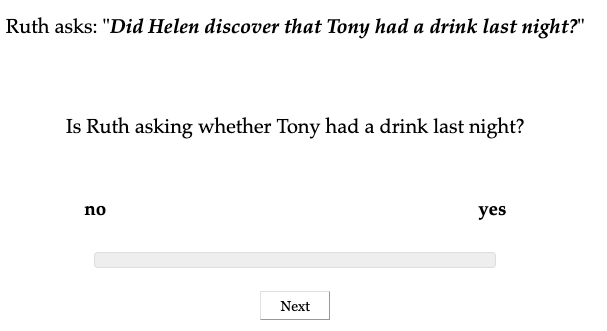
\includegraphics[width=\linewidth]{../../writing/paper/figures/trialExp5}}
				&
				\visible<2->{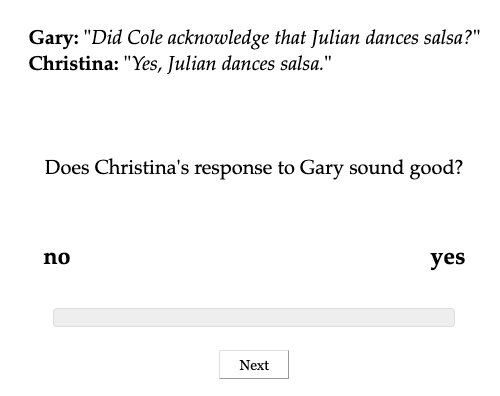
\includegraphics[width=\linewidth]{../../writing/paper/figures/trialExp6}}
				\\
				
			\end{tabular}
		\end{center}\pause

		Across both experiments, 550 participants saw each of 20 conditions once, each randomly paired with a clause to instantiate it (item), e.g. \emph{Julian dances salsa} + 6 control trials (attention checks)

	\end{frame}


	\begin{frame}[t]\frametitle{Results}\scriptsize

	      \centering
	      \begin{tabular}{p{.48\linewidth} p{.48\linewidth}}
	      	Exp.~5 (`asking whether' diagnostic)
	      	&
	      	Exp.~6 (`direct response' diagnostic)\\ 
	      	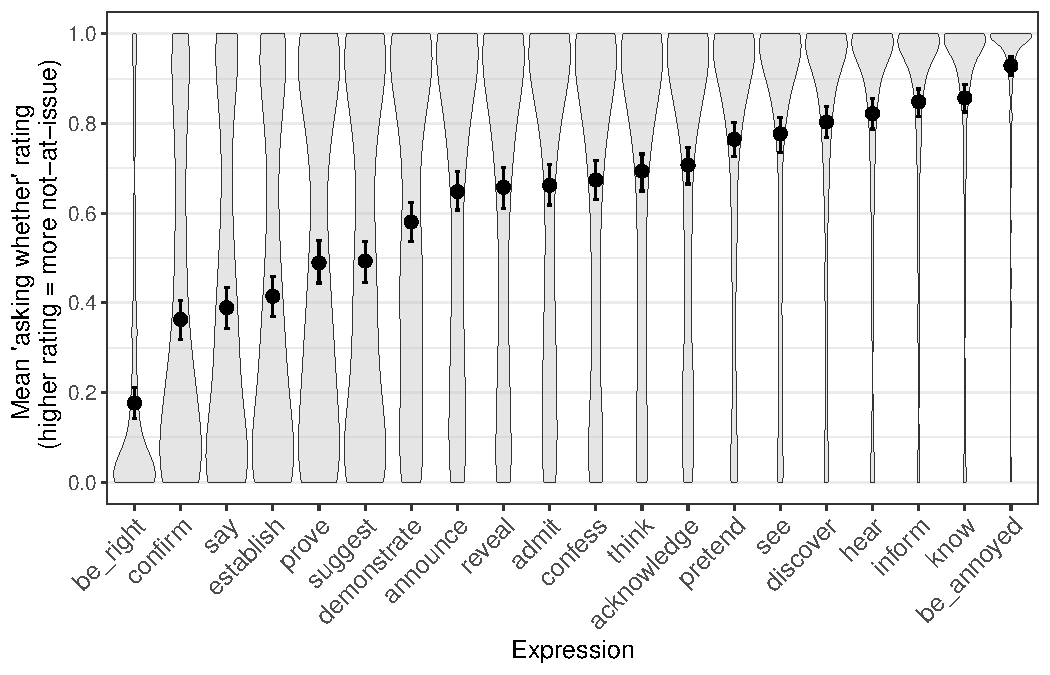
\includegraphics[width=\linewidth]{../../results/exp5/graphs/mean-ratings.pdf}%
	      	&
	      	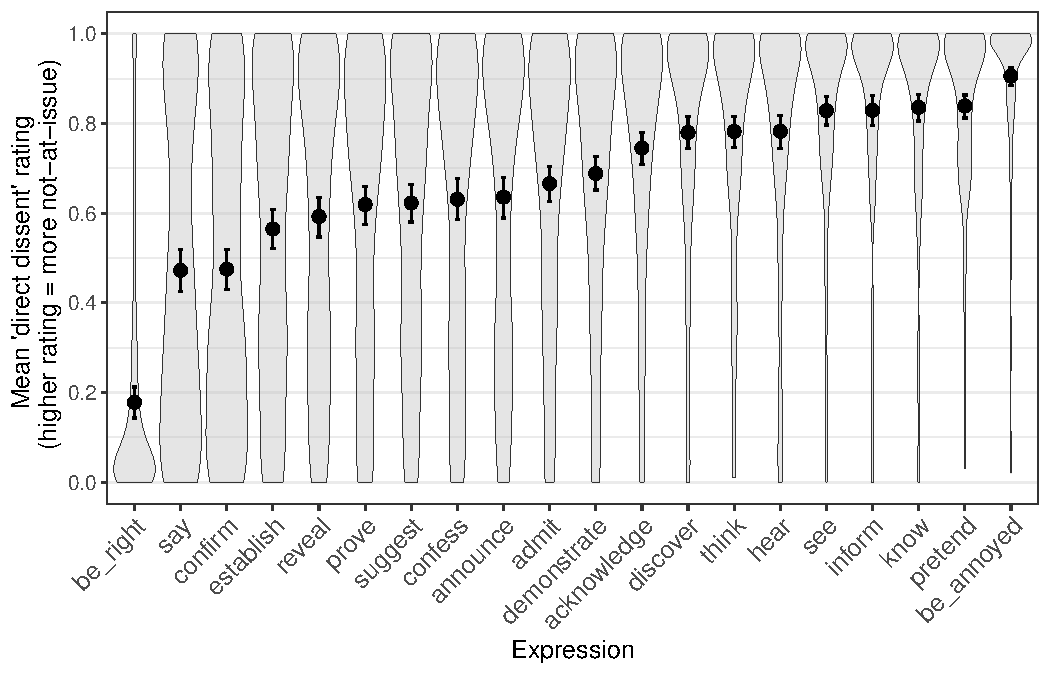
\includegraphics[width=\linewidth]{../../results/exp6/graphs/mean-ratings.pdf}
	      	\\
	      \end{tabular}\pause

	      % Results of Exps.~5-6. The panels show the mean ratings by expression for (a) Exp.~5 (asking whether diagnostic) and (b) Exp.~2 (direct assent diagnostic). Error bars indicate 95\% bootstrapped confidence intervals. Violin plots show the kernel probability density of individual participants' ratings.
	      \vfill

	      \begin{itemize}
	      	\item Results look very similar here
	      	\item Pairwise differences bteween many of the same contents (?)\pause
	      	\item By-content means from the two experiments are highly correlated (Spearman rank correlation = .93)
	      \end{itemize}
	
	\end{frame}

	\begin{frame}\frametitle{Discussion}
		
		\begin{itemize}
			\item Results from Exps.~5–6 are highly correlated 
			\item The speech act (question vs. assertion) matters most for how sensitive a diagnostic is to differences between contents
			\begin{itemize}
				\item More than response task
				\item More than question-based vs. assertion-based diagnostics
			\end{itemize}
		\end{itemize} \vfill \pause

		{\scriptsize Different from previous literature suggesting that different diagnostics show different empirical results:\\
		Mostly higlighted difference between QUD at-issueness, and assertion-based diagnostics, which are either argued not to be about at-issueness at all (\citealt{snider_anaphoric_2017,snider_at-issuenessne_2017,snider_distinguishing_2018}), or about a separate assertion-based notion of at-issueness (\citealt{koev_notions_2018,faller_discourse_2019,korotkova_evidential_2020})}

	\end{frame}	

\section{General discussion}

	\begin{frame}[t]\frametitle{Question embeddings}\small 
		So why are question embeddings so different from assertions? Some speculation:\pause

		\begin{itemize}[<+->]
			\item \textbf{Literal meaning} of appositives / lexical semantics of clause-embedding verbs affects how much/likely the embedded content is interpreted as at issue\\ 
			{\scriptsize Big question here: which lexical properties can affect this how? Look to literature on presupposition triggering? (\citealt{abrusan_predicting_2011,schlenker_triggering_2021,anand_facts_2024}, Scontras \& Tonhauser to appear)}

			\item \textbf{Questions:} At-issue content introduces a question partition, but no speaker commitment

			\item \textbf{Projection:} In any context, not-at-issue content projects, and we understand the speaker to be committed to it

			\item \textbf{Assertions:} Speaker is committed to the at-issue content as well, and therefore at-issue content and not-at-issue content are harder to distinguish

			\item Therefore \textbf{questions are good context to test at-issueness differences} which may be conditioned by literal
			% (and maybe directive speech acts)

			\item Testing the at-issueness of contents in declarative assertions muddles the picture, making at-issue and not-at-issue content harder to distinguish; especially when the test itself invokes commitment (like those using assent/dissent)

		\end{itemize}
	
	\end{frame}
	
	\begin{frame}\frametitle{Takeaways}
	
		\begin{itemize}[<+->]
			\item Experimental confirmation for claims that there are empirical differences between at-issueness diagnostics (\citealt{snider_anaphoric_2017,snider_at-issuenessne_2017,snider_distinguishing_2018,koev_notions_2018,faller_discourse_2019,korotkova_evidential_2020})
			\begin{center}
				\textbf{It matters which diagnostic is used.}\bigskip
			\end{center}


			\item But: difference between QUD at-issueness and assertion-based diagnostics does not seem to be the most important; \textbf{speech act} where the target content is embedded is more important \medskip

			\item No replication of \citealt{syrett_experimental_2015}: We did not find that final appositives are more at-issue than medial ones
			\medskip

			\item Left open here: What the results might tell us about whether the diagnostics reflect a shared underlying notion of at-issueness
		\end{itemize}

		% \begin{itemize}
			% 	\item these are not relative to a QUD-notion of at-issueness \citealt{snider_anaphoric_2017,snider_at-issuenessne_2017,snider_distinguishing_2018,koev_notions_2018,faller_discourse_2019,korotkova_evidential_2020}
			% 	\item Snider: not about at-issueness at all
			% 	\item Murray: p-at-issueness
			% \end{itemize}
	
	\end{frame}



\begin{frame}[allowframebreaks]{\bfseries\opt References}
	\footnotesize
	\bibliographystyle{../cslipubs-natbib}
	\bibliography{../../writing/at-issueness}

\end{frame}

\end{document}